\chapter{Introduction}



The fraction of irradiation reflected by Earth's surface is called the albedo. It is linked with the composition and properties of the surface and, therefore varies throughout the year. The average albedo for our planet Earth is between $0.1$ and $0.3$. Using "ERA5-Land monthly averaged data from 1950 to present" from the Copernicus Datastore \cite{hersbach2020era5}, it is possible to retrieve the variable "forecast albedo", which is defined as \textit{the fraction of solar (shortwave) radiation reflected by Earth's surface, across the solar spectrum, for both direct and diffuse radiation}. The figure \ref{fig:avg_albedo} represent monthly averaged albedo value from 1993 to 2022.  

\begin{figure}[ht]
	\centering
	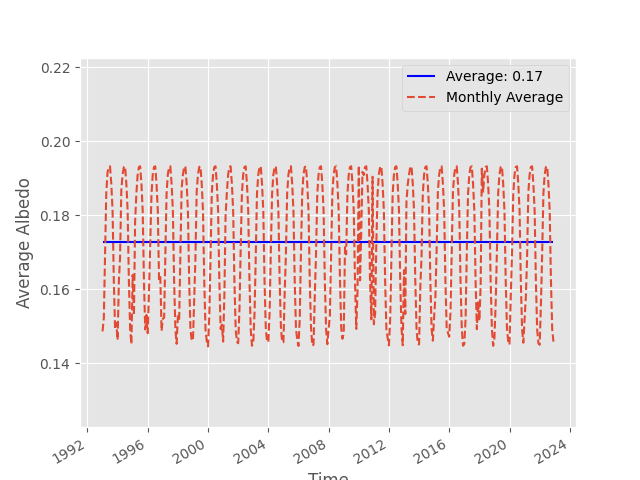
\includegraphics[width=8cm]{albedo_avg_clim}
	\caption{Average value over Ireland from 1993 to 2022}
	\label{fig:avg_albedo}
\end{figure}


The meaning of this graphic above, is to show the variation of the albedo over the last $30$ years in Ireland around a average value of $0.17$. Under normal circumstance, the albedo hits a maximum during winter and falls back to a minimum during summer. During winter, snow appears which increases the amount of reflected radiation. The last week of $2010$, famously covered the majority of the land in snow, which result in a anomalously high value of the albedo as explained by \cite{garciaclimate2021}. 



\begin{figure}[ht]
	\centering
	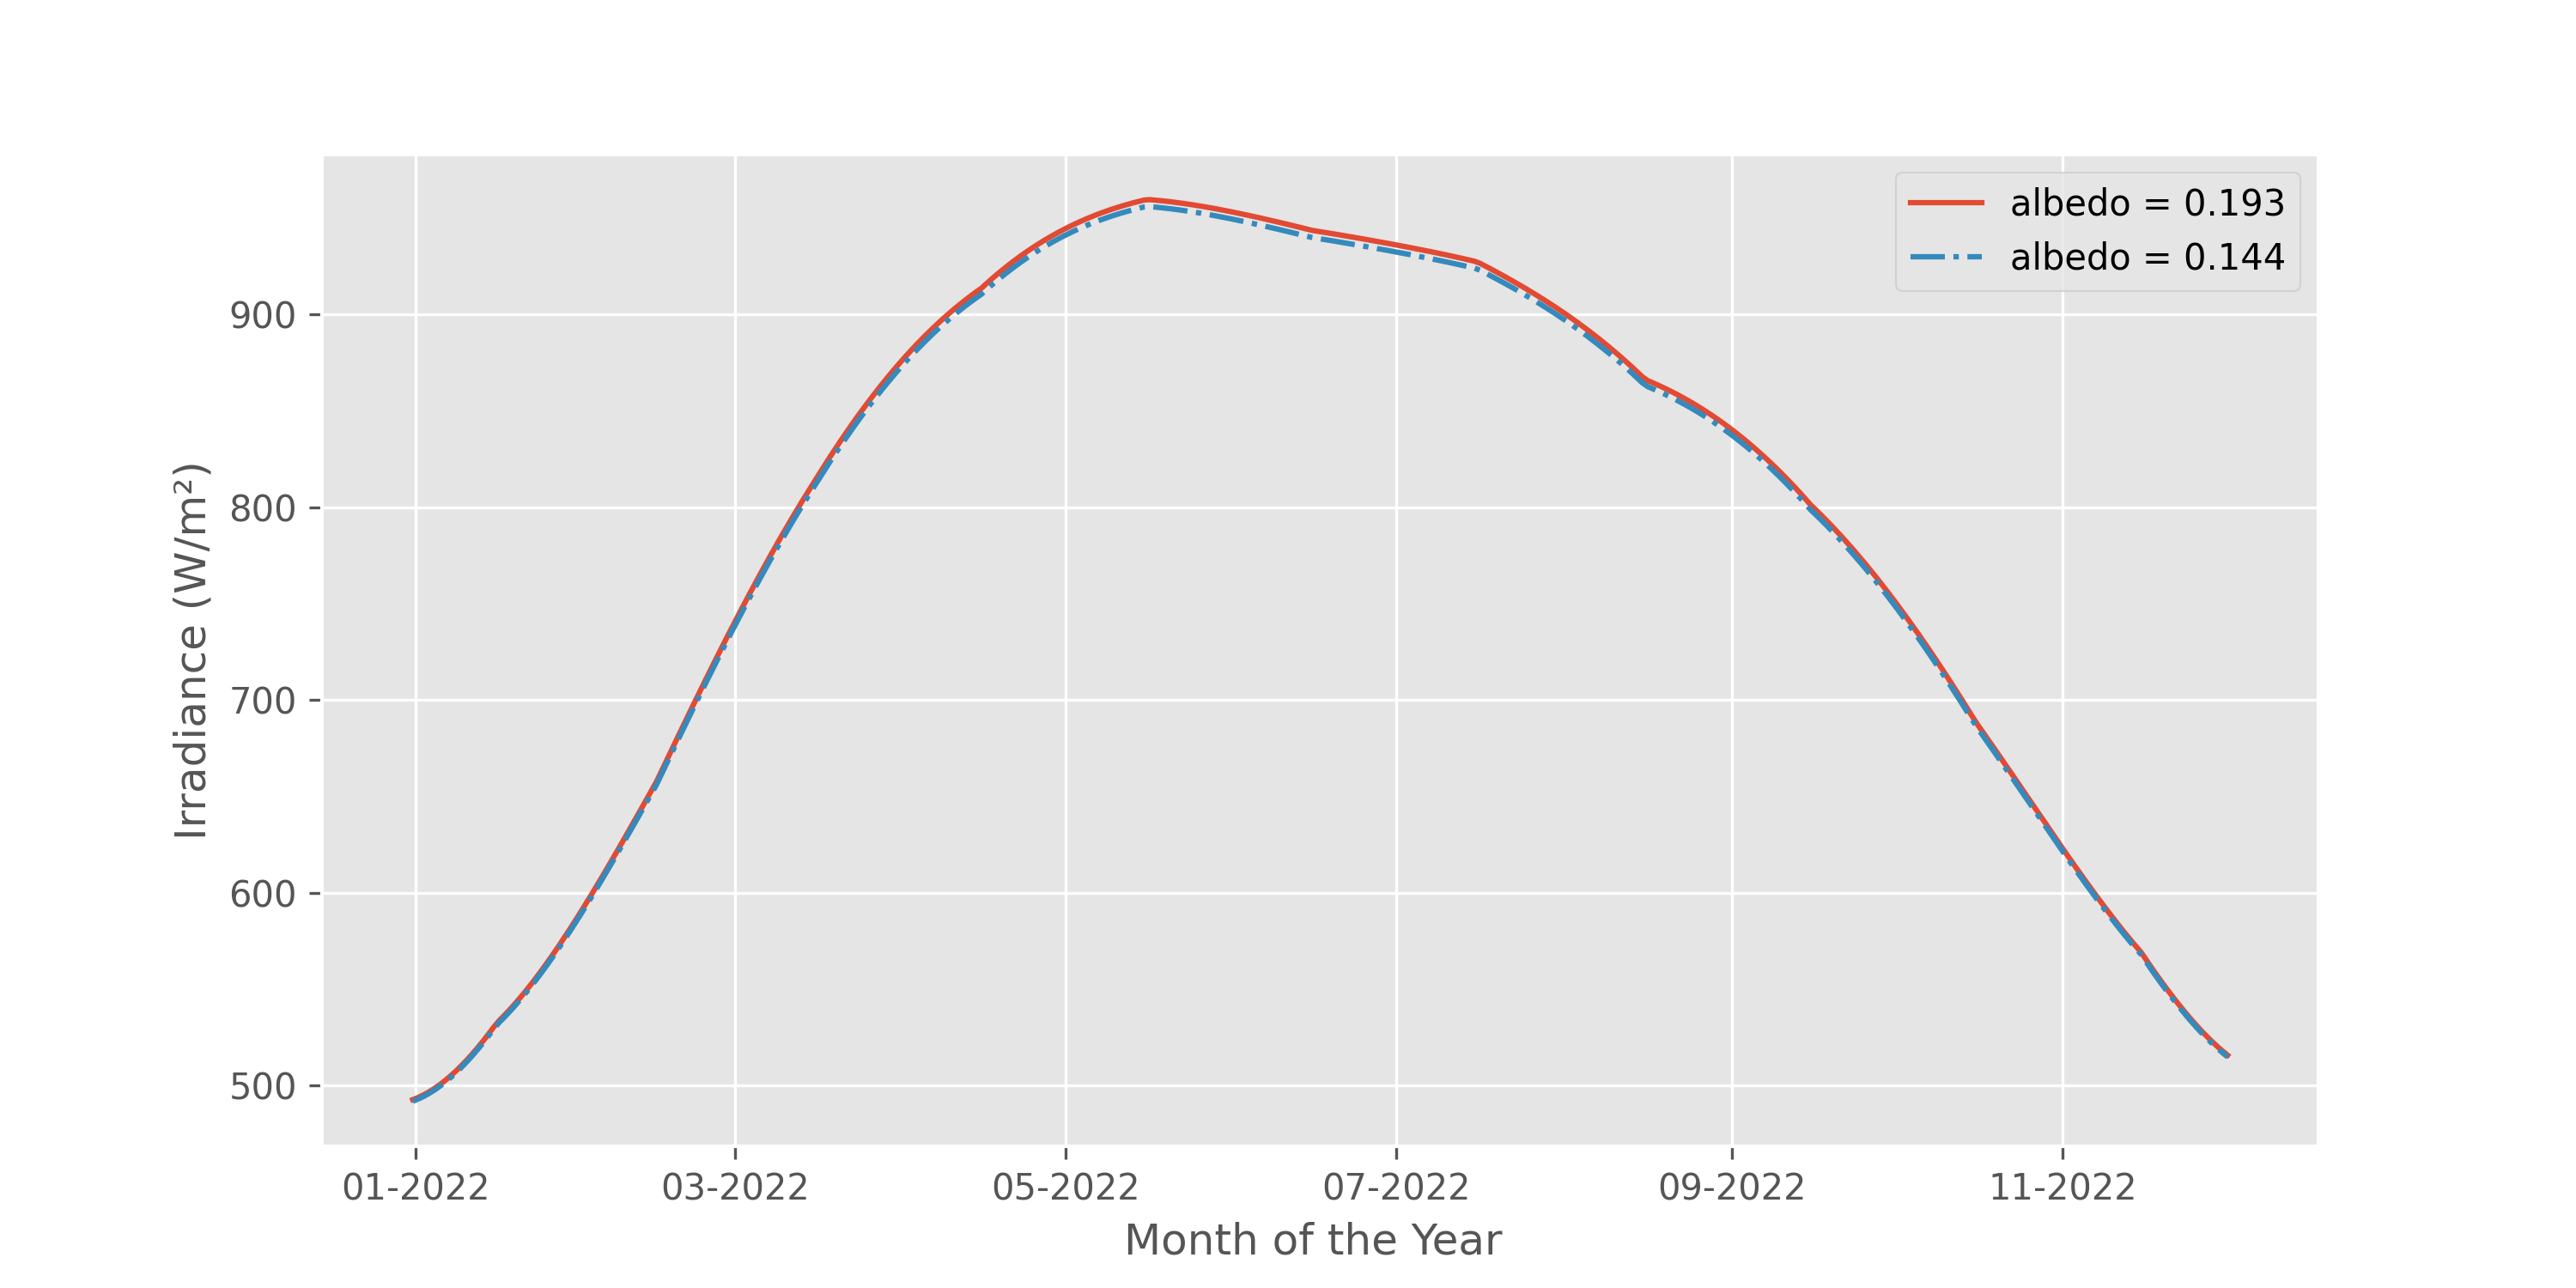
\includegraphics[width=8cm]{Diff_POA_Albedo.png}
	\caption{Difference of the global irradiance on a module plane for two extrems albedos at 12:00}
	\label{fig:irradiance_albedo}
\end{figure}